%!TEX root = ../main-anran-ma.tex 
% so I can build in this tex file too. 
%*****************************************
\chapter{Preliminaries}\label{ch:Preliminaries}
%*****************************************
% \setcounter{theorem}{0}
% \NoCaseChange{Homo Sapiens}
\setcounter{figure}{0}


\section{Notations}\label{sec:notation}
Before proceeding, we clarify the notations used in this thesis, which are not uncommon in materials of computer science and mathematics. 
Readers are encouraged to skip this section and refer back to it if needed. 
The notations and their meaning are listed in \autoref{tab:notation}. 

\begin{table}[ht]\centering
    \begin{tabular}{@{}l;{1pt/1pt}l@{}}
      \hline \hline
      \textbf{Notation}  & \textbf{Meaning} \\\hline
      $\X$     &  set of program variables \\ \hdashline[1pt/1pt]
      $\V$   & set of values\\ \hdashline[1pt/1pt]
      $s:\X\rightarrow\V$   &  program states \\\hdashline[1pt/1pt]
      $\S$  &  set of program states \\\hdashline[1pt/1pt]
      $\C$  &  set of programs \\\hdashline[1pt/1pt]
      $\P$  &  set of predicates \\\hdashline[1pt/1pt]
      $F : \S\rightarrow \{true, false\}$  &  predicates \\
      $F:=\{\sigma\in\S\mid F(\sigma)\}$ \hypertarget{2.*}{(*)} &  the set described by a predicate \\ \hdashline[1pt/1pt] 

      \begin{tabular}{@{}l}
        $F(\sigma)$ \hypertarget{2.**}{(**)}\\
        $F(\sigma) = true$ (**)\\ 
        $\sigma\vDash F$   \\
        $\sigma\in F$  
      \end{tabular}        &  
      \begin{tabular}{@{}l}
        state $s$ satisfies predicate $F$; \\
        $F$ is true when system is in state $\sigma$
      \end{tabular}    \\  \hdashline[1pt/1pt]  

      $\sigma\goto{c}\tau$   & 
      \begin{tabular}{@{}l}
        from initial state $\sigma$, an execution of program $c$ \\ 
        terminates at final state $\tau$ 
      \end{tabular}    \\  \hdashline[1pt/1pt] 

      $\sigma\goto{c}\bot$  & 
      \begin{tabular}{@{}l}     
        from initial state $\sigma$, an execution of program $c$ \\ 
        diverges
      \end{tabular}    \\  \hdashline[1pt/1pt] 
      
      \begin{tabular}{@{}l}     
        $\exists x . P : F $\\ 
        $\forall x . P : F $
      \end{tabular} 
      & there exists/for all $x$ such that $P$ is true: $F$ is true
      \\

      \hline\hline
    \end{tabular}
    \caption{Symbols and Notations}
    \label{tab:notation}
\end{table}

It is worth noting that we regard program states as total functions - we assume that we can assign some default values to variables in case they are undefined. 
We also simplify matters by assuming that there is only one interpretation as a total function from predicates to truth values. 
As a result, we can regard predicates as (total) functions from program states to truth values. 
We also overload the symbols for predicates and use them to identify the sets they describe as shown in \hyperlink{2.*}{Line (*)}. 

By default, we take \mathl{F(\sigma)} to mean the same as \mathl{F(\sigma)= true} for convenience's sake as shown in \hyperlink{2.**}{Lines (**)}. 
We also omit the use of equivalence symbol ``\mathl{\equiv}'' since we always use ``\mathl{:=}'' while defining objects, so we simply use the equation symbol ``\mathl{=}'' for equivalences instead. 
Now we can proceed to discuss proof rules and systems that are relevant for this thesis. 




\section{Hoare Logic}
Since the beginning of the 1960s, scholars have been researching the establishment of mathematics in computation~\cite{floyd93, mccarthy93} to have a formal understanding and reasoning of programs. 
One of the most known methods is \define{Hoare logic}. 

In 1969, C.A.R. Hoare wrote \textit{An Axiomatic Basis for Computer Programming}~\cite{hoare69} to explore the logic of computer programs using axioms and inference rules to prove the properties of programs. 
He introduced \imptt{sufficient} preconditions that  guarantee correct results but do not rule out non-termination. 
A selection of the axioms and rules are shown in~\autoref{tab:hoare}.~\footnote{We omit the symbol $\vdash$ in front of a Hoare triple, which denotes ``valid/provable'', for better readability. }\footnote{Non-determinism was not considered in the original paper, so we treat the programs here as deterministic. 
With deterministic programs, one initial state corresponds to one final state, and in case of non-termination we assign a final state $\bot$. }

\todo{Think about whether to add liberally deterministic (Hesselink 1992, Programs, Recursion and Unbounded Choice). }

\mathl{\{F[x/e]\}} is obtained by substituting occurrences of $x$ by $e$. 

\begin{table}[ht]\centering
    \begin{tabular}{l;{1pt/1pt}l}
      \hline \hline
      \textbf{Axiom of Assignment}     &  \hoare{F[x/e]}{x:=e}{F}   \\ \hdashline[1pt/1pt]
      \textbf{Rules of Consequence}   &  If \hoare{G}{C}{F} and $F\Rightarrow P$ then \hoare{G}{C}{P} \\
                                      &  If \hoare{G}{C}{F} and $P\Rightarrow G$ then \hoare{P}{C}{F} \\ \hdashline[1pt/1pt]
      \textbf{Rule of Composition}   &  If \hoare{G}{C_1}{F_1} and \hoare{F_1}{C_2}{F} then \hoare{G}{C_1;C_2}{F} \\\hdashline[1pt/1pt]
      \textbf{Rule of Iteration}  &  If \hoare{(F\wedge B)}{C}{F} then \hoare{F}{\text{while } B \text{ do } C }{\neg B \wedge F}  \\
      % \textbf{Rule of Condition}   &  $wp.C_1.(wp.C_2.F)$\\
      \hline\hline
    \end{tabular}
    \caption{Inference Rules for Valid Hoare Triple}
    \label{tab:hoare}
\end{table}

Semantically, a Hoare triple {{\mathl{\hoarenm{G}{C}{F}}}} is said to be valid for (partial) correctness, if the execution of the program $C$ with an initial state satisfying the precondition $G$ leads to a final state that satisfies the postcondition $F$, provided that the program terminates. 
The definitions in \autoref{tab:hoare} indeed correspond to this intended semantics. Formal soundness proofs can be found in Krzysztof R. Apt's survey~\cite{apt81} in 1981.
As an example, consider the rule of composition: if the execution of program $C_1$ changes the state from $G$ to $F_1$, and $C_2$ changes the state from $F_1$ to $F$, then executing them consecutively should bring the program state from $G$ to $F$, with the intermediate state $F_1$.

The missing guarantee of termination can be seen in the rule of iteration: consider the triple {\mathl{\hoarenm{x\leq 2}{\text{while } x\leq 1 \text{ do } x:=x*2}{1<x\leq 2}}}, it is provable in Hoare logic with the following proof tree. 
However, this while-loop will not terminate in case $x\leq 0$ in the initial state.
\begin{center}
\colorbox{ForestGreen!5}{
\begin{prooftree}
  \infer0[\ \ \textbf{Axiom of Assignment}]{\hoarenm{x\leq 1}{x:=x*2}{x\leq 2}}
  \infer1[\ \ \textbf{Rule of Iteration}]{\hoarenm{x\leq 2}{\text{while } x\leq 1 \text{ do } x:=x*2}{1<x\leq 2}}
\end{prooftree}}
\end{center}

Using style taken from Benjamin L. Kaminski's dissertation~\cite{kaminski19}, \autoref{fig:hoare} illustrates a valid Hoare triple: $\S$ represents the set of all states, the section denoted with $G$ includes the states that satisfy the predicate $G$. 
The arrows from left to right denote the executions of program $C$. 
The dashed arrows denote non-terminating executions. 

\begin{figure}[ht!]\centering
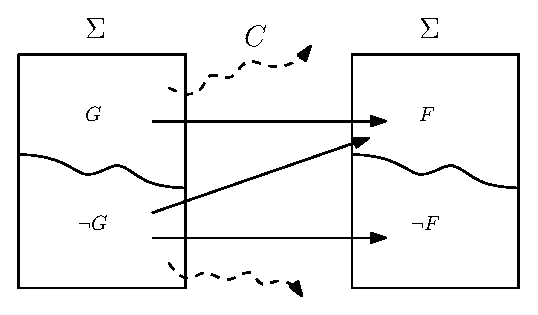
\includegraphics[width=0.5\textwidth]{image/hoare.eps}
\caption{Valid Hoare Triple (Deterministic)}
\label{fig:hoare}
\end{figure}


A sensible advancement of Hoare logic would be to also prove termination, i.e. to eliminate the arrows from $G$ to the abyss.  
Supplementing Hoare logic with a termination proof is done by Zohar Manna and Amir Pnueli in 1974~\cite{manna74}, where they introduced what we call a \define{loop variant}, a value that decreases with each iteration. The name is in contrast to \define{loop invariant}, concretely the $F$ in \textbf{Rule of Iteration} in \autoref{tab:hoare}, which is constant before and after the loop. 

Another advancement would be to find the \imptt{necessary and sufficient} preconditions that grant us the post-properties, i.e. to eliminate the arrows from $\neg G$ to $F$ in \autoref{fig:hoare}, which  is what Edsger W. Dijkstra accomplished with his \define{weakest precondition} transformer in 1975~\cite{dijkstra75}, among other things. 


\section{Guarded Command Language}\label{sec:gcl}
From now on we will use Dijkstra's (non-deterministic) \define{guarded command language (GCL)}~\cite{dijkstra75} to represent programs and to include non-determinism (starting from \autoref{sec:wp-nondet}).
For better readability, we use an equivalent\footnote{Specifically, \mathl{if\ (\varphi)\ \{C_1\}\ else\ \{C_2\}}  is equivalent to
\mathl{if\ \varphi \to C_1\ []\ \neg\varphi \to C_2\ fi} in Dijkstra's original style~\cite{dijkstra75}; \mathl{\{C_1\}\square \{C_2\}} is equivalent to \mathl{if\ true\to C_1\ []\ true\to C_2\ fi}.} 
form of GCL that is similar to modern pseudo-code as shown in \autoref{tab:gcl}. 


\begin{table}[ht!]\centering
    \begin{tabular}{clll}
    $C\ ::=$ 
      & $x:= e$ &  $\mid \ C;C $ & $\mid\  \{C\}\square \{C\} $ \\
      &\footnotesize\define{assignment} &\footnotesize\define{sequential composition} 
      & \footnotesize\define{non-deterministic choice} \\
      &$\mid\  if\ (\varphi)\ \{C\}\ else\ \{C\}$ & $\mid\ while\ (\varphi)\ \{C\}$
      &$\mid\ skip \ \ \ \ \mid\ diverge$ \\ 
      &\footnotesize\define{conditional choice} &\footnotesize\define{while-loop} 
    \end{tabular}
    \caption{Guarded Command Language}
    \label{tab:gcl}
\end{table}

The \define{assignment, sequential composition, conditional choice, while-loop} commands conform to their usual meaning.
The \define{non-deterministic choice} \mathl{\{C_1\}\square \{C_2\}} chooses from two programs randomly. 
It is however not \define{probabilistic}, meaning we do not know the probabilistic distribution of the outcome of the choice. 

When \mathl{skip} is executed, the program state does not change and the consecutive part is executed. 
When \mathl{diverge} is executed, the program goes to a state symbolizing non-termination, and the execution stops. 

In our representation of GCL, non-determinism is explicitly constructed via the infix operator \mathl{\square}, whereas in its original definition, non-determinism occurs when the guards within the \mathl{if} and \mathl{while} commands are not mutually exclusive~\cite{dijkstra90}. 
Additionally, the \mathl{if} statement in Dijkstra's GCL is equivalent to divergence in case non of its guards are true, but in our version this can no longer happen because of the Law of Excluded Middle: the predicate $\varphi$ must be either true or false, so either the ``then'' branch or the ``else'' branch is activated.
Consequently, non-termination can only originate from either the \mathl{diverge} or the \mathl{while} command. 


\section{Weakest Preconditions}\label{sec:wp}

\subsection{The Deterministic Case}\label{sec:wp-det}
To better relate Hoare triples and Dijkstra's weakest precondition transformer, we first focus on deterministic programs. 
The goal is to find the \imptt{necessary and sufficient} precondition such that the program is guaranteed to \imptt{terminate} in a state that satisfies the postcondition. 
\autoref{fig:hoare-wp-det} shows it graphically alongside the figure for valid Hoare triples. 
We can see that in \autoref{subfig:wp-det}, the arrows from $G$ to non-termination and from $\neg G$ to $F$ are absent. 

\begin{figure}[ht!]\centering
  \subfloat[Valid Hoare Triple \label{subfig:hoare}]{
    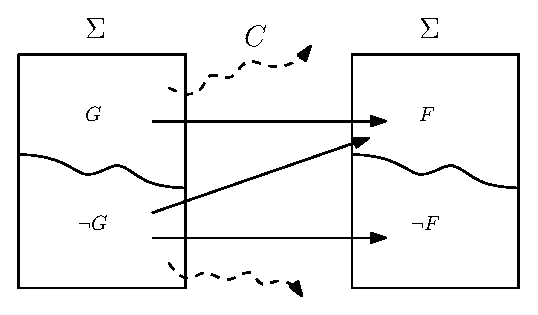
\includegraphics[width=0.45\textwidth]{image/hoare.eps}
  }
  \hfill
  \subfloat[Weakest precondition \label{subfig:wp-det}]{
    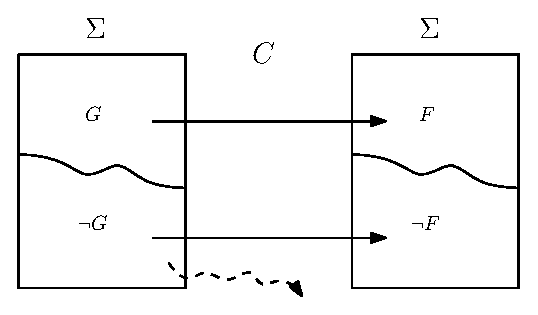
\includegraphics[width=0.45\textwidth]{image/wp-det.eps}
  }
\caption{Valid Hoare Triple vs. Weakest Precondition (Deterministic)}
\label{fig:hoare-wp-det}
\end{figure}

We define the \define{weakest precondition} transformer inductively over the program structure in lambda-calculus style\footnote{For example, $wp.C.F$ can be seen as $wp(C,F)$ in ``typical'' style, where wp is treated as a function that has two parameters. The advantage of lambda-calculus style is scalability, we can simply extend the aforementioned function to $wp.C.F.\sigma$ where $\sigma$ means the initial state. Here wp is treated as a function that has three parameters, if we were to write it in the ``typical'' style. It is then questionable whether we changed the type of wp. } as in \autoref{tab:wp-det}: 

\begin{table}[ht!]\centering
    \begin{tabular}{l;{1pt/1pt}l}
    \hline\hline
      \textbf{C}&\textbf{wp.C.F}    \\ \hline
      $skip$&   $F$   \\ \hdashline[1pt/1pt]
      $diverge$&  $false$\\ \hdashline[1pt/1pt]
      $x:= e $&  $F[x/e]$\\ \hdashline[1pt/1pt]
      $C_1;C_2$&  $wp.C_1.(wp.C_2.F)$\\ \hdashline[1pt/1pt]
      $if\ (\varphi)\ \{C_1\}\ else\ \{C_2\} $&  $(\varphi\wedge wp.C_1.F)\vee(\neg\varphi\wedge wp.C_2.F)$\\ \hdashline[1pt/1pt]
      % $\{C_1\}\square \{C_2\}$ & $wp.C_1.F\vee wlp.C_2.F$ \\
      $while\ (\varphi)\ \{C'\}$&  $lfp\ X.(\neg\varphi\wedge F)\vee(\varphi\wedge wp.C'.X)$\\
    \hline\hline
    \end{tabular}
    \caption{The Weakest Precondition Transformer for Deterministic Programs~\cite{kaminski19}}
    \label{tab:wp-det}
\end{table}

\mathl{F[x/e]} is $F$ where every occurrence of $x$ is syntactically replaced by $e$. 

\mathl{lfp\ X. f} is the least fixed point of function $f$ with variable $X$. 

Let {$$\Phi(X):=(\neg\varphi\wedge F)\vee(\varphi\wedge wp.C'.X)$$} be the characteristic function, then wp for while-loop can be defined as: 
{$$wp.(while(\varphi)\{C'\}).F = lfp\ X. \Phi(X)$$}

Most of the definitions in \autoref{tab:wp-det} are intuitive and correspond to their counterparts in Hoare logic, while those for \mathl{diverge} and \mathl{while} deserve special attention. 
Since wp aims for total correctness, a program starting in an initial state satisfying the precondition \mathl{wp.diverge.F} should terminate in a final state satisfying the postcondition \mathl{F}. 
Because \mathl{diverge} does not terminate, there is no such precondition and wp for \mathl{diverge} should be \mathl{false}. 

The definition for the while-loop~\cite{kaminski19} is trickier, but we can verify its correctness by recalling Dijkstra's original definition in the following section. 

%\solved{Find out if there's earlier definition that used lfp. -> yes, dijkstra&scholten}

\subsection{Defining Loops}\label{sec:define loops}
In Dijkstra's original paper~\cite{dijkstra75}, he defined wp for while-loops based on its (intended) semantics, i.e. the precondition that guarantees loop termination with the required postcondition within a certain number of iterations. 

Let 
\[
WHILE=while(\varphi)\{C'\}
\\\text{ and } \\ 
IF=  if\ (\varphi)\{C'\}\ else\ \{diverge\}. 
\] 
%\footnote{In our model, the if construct have only one guard $\varphi$, which if written in the original style would be $if \varphi \to C'$ }
Rewriting Dijkstra's definition in a form conforming to our style, he defines 
\[
H_0(F)=( \neg \varphi\wedge F )
\\\text{ and } \\ 
H_k(F)=wp.IF.H_{k-1}(F) \vee H_0(F). 
\]

\mathl{IF} is defined in such way that $wp.IF.X$ is the weakest precondition that makes sure the guard of \mathl{IF} discharges and $C'$ is executed once, leaving the program in a state satisfying $X$.
As a result, $H_k(F)$ corresponds to the weakest precondition such that the program terminates in a final state satisfying $F$ after \imptt{at most} $k$ iterations.


%done{Explain a bit more about how this relate to the above definition. }

Then by definition: 
\begin{equation}
  \hspace{2.5cm}wp.WHILE.F=(\exists k\geq 0: H_k(F)) \label{eq:while}
\end{equation}

The definition in \autoref{tab:wp-det}, however, uses the least fixed point of the characteristic function that is not obvious. 
We understand the use of fixed point in two ways. 
First, a precondition $G$ being a fixed point of the characteristic function $G= \Phi(G)=(\neg\varphi\wedge F)\vee(\varphi\wedge wp.C'.G)$ means that under control of $G$, termination is possible (left side of the disjunction) and repeated execution of $C'$ is possible(right side of the disjunction), since $G$ is invariant before and after the execution of $C'$. 
Second, if we were to believe that the semantics of $WHILE$ should be equivalent to the semantics of $if(\varphi)\{C;WHILE\}else\{skip\}$, we can derive the need for fixed point: 
\begin{align*} 
  wp.WHILE.F    & \seq wp.(\text{if }(\varphi)\{C;WHILE\}\text{ else }\{skip\}.F) \\
                & \seq \varphi\wedge wp.(C;WHILE).F \vee \neg\varphi\wedge wp.skip.F\\ 
                & \seq \varphi\wedge wp.C.(wp.WHILE.F) \vee \neg\varphi\wedge F\\ 
                & \seq \Phi(wp.WHILE.F)\\ 
\end{align*}

The question then arises: can we define wp with any fixed point? 
The answer is no and we show it by verifying that the definition in \autoref{tab:wp-det} coincides with Dijkstra's definition at the beginning of this chapter.\footnote{In fact, Dijkstra and Scholten\cite{dijkstra90} later also gave definitions for wp and wlp in an equivalent form of least and greatest fixed points, they called it "strongest" and "weakest solution". They also proved that it is necessary to use the extreme solutions. }
We borrow a theorem from domain theory that yields a computation for least fixed points, provided they exist: 
\begin{theorem}{lfp}
hello test 
\textbf{[Insert theorem]}%TODO

\end{theorem}


Coincidentally, $H_k(F)$ is the $(k+1)-$th iteration of the characteristic function $\Phi$ from the bottom element, denoted by $\Phi^{k+1}(false)$. 
For all predicates $F$ and all programs $C'$: 
\begin{lemma}{hk-phi}
$\forall k\geq 0: H_k(F)=\Phi^{k+1}(false)$
\end{lemma}

\begin{proof}
Proof by induction. 
\vspace{-0.25cm}\paragraph{Base case: } 
  \begin{align*} 
    \Phi(false)   & = (\neg\varphi\wedge F)\vee(\varphi\wedge wp.C'.false)  & \\ 
                  & = (\neg\varphi\wedge F)\vee(\varphi\wedge false)         && |\ \hypertarget{2.***}{\text{(***)}}\\
                  & = \neg\varphi\wedge F                                    && |\ \text{predicate calculus} \\
                  & = H_0(F)
  \end{align*}
\hyperlink{2.***}{Line (***)} is supported by the Law of Excluded Miracle~\cite[p.18]{dijkstra76}: for all programs $C$, $wp.C.false = false$. 
It states that it is impossible for a program to terminate in a state satisfying no postcondition. 

\vspace{-0.25cm}\paragraph{Step case: } 
  \begin{align*} 
    H_{k+1}(F)     & = wp.IF.H_{k}(F) \vee H_0(F) \\
                  & = (\varphi\wedge wp.C'.H_{k}(F))\vee(\neg\varphi\wedge wp.diverge.H_{k}(F)) \vee H_0(F) \\ 
                  &\hspace{0.45\textwidth} | \ \text{unfold IF; definition of wp} \\
                  & = (\varphi\wedge wp.C'.H_{k}(F))\vee(\neg\varphi\wedge false) \vee H_0(F) \\
                  &\hspace{0.45\textwidth} | \ \text{definition of wp} \\
                  & = (\varphi\wedge wp.C'.\Phi^{k+1}(false)) \vee H_0(F)  \\
                  &\hspace{0.45\textwidth} | \ \text{induction hypothesis} \\
                  & = (\varphi\wedge wp.C'.\Phi^{k+1}(false)) \vee (\neg\varphi\wedge F)  \\
                  & = \Phi^{k+2}(false)  \\
  \end{align*}

\end{proof}

Thus by identifying the least fixed point, we find a $k$ that satisfies \autoref{eq:while}.
The advantage of using least fixed point to define wp is that there are heuristics to find it, whereas \autoref{eq:while} excels at giving intuitions for the preconditions that guarantee loop termination. 
Essentially, they express the same predicate, i.e. the ``weakest'' precondition for while-loops which is unique. 
Consequently, it means that we can not use other fixed points to define $wp.WHILE$, which are weaker than the least fixed point. 
For the same reason, we will see that greatest fixed point is necessary to define weakest liberal precondition. 


\subsection{The Non-deterministic Case: Angelic vs. Demonic}\label{sec:wp-nondet}
Now we bring the non-deterministic choice back into the picture and add its wp to \autoref{tab:wp-wlp}. 
Here we assume a setting with \define{angelic non-determinism}, where we assume that whenever non-determinism occurs, it will be resolved in our favor.
This results in the weakest precondition for our non-deterministic choice being a disjunction of the wp for its subprograms. 
We are hopeful that a precondition satisfying the wp of one of the subprograms can also lead to termination in our desired postcondition. 
This is a design choice that is different from Dijkstra's~\cite{dijkstra75}, where the wp for non-deterministic choice is a conjunction, hinting at a demonic setting. 
Both choices are justifiable, we choose to follow Zhang and Kaminski's work, favoring the resulting Galois connection between the weakest (liberal) precondition transformers and the strongest (liberal) postcondition transformers~\cite{zhang22}. 


\begin{table}[ht!]\centering
    \begin{tabular}{l;{1pt/1pt}l;{1pt/1pt}l}
    \hline\hline
      \textbf{C}&\textbf{wp.C.F} & \textbf{wlp.C.F}   \\ \hline
      $skip$&   $F$ &   $F$   \\ \hdashline[1pt/1pt]
      $diverge$&  $false$&  $true$\\ \hdashline[1pt/1pt]
      $x:= e $&  $F[x/e]$&  $F[x/e]$\\\hdashline[1pt/1pt]
      $C_1;C_2$&  $wp.C_1.(wp.C_2.F)$&  $wp.C_1.(wp.C_2.F)$\\\hdashline[1pt/1pt]

      {\color{Maroon}$\{C_1\}\square \{C_2\}$} & {\color{Maroon}$wp.C_1.F\vee wp.C_2.F$} & {\color{Maroon}$wlp.C_1.F\wedge wlp.C_2.F$}\\\hdashline[1pt/1pt]

      $if\ (\varphi)\ \{C_1\} $ &  $(\varphi\wedge wp.C_1.F)$ &  $(\varphi\wedge wp.C_1.F)$\\
      $\ \ \ \ \ \ \ \  else\ \{C_2\} $&  $\ \ \ \ \ \ \ \ \vee(\neg\varphi\wedge wp.C_2.F)$ &  $\ \ \ \ \ \ \ \ \vee(\neg\varphi\wedge wp.C_2.F)$\\\hdashline[1pt/1pt]

      {\color{Maroon}$while\ (\varphi)\ \{C'\}$} &  $lfp\ X.\ (\neg\varphi\wedge F)$ & {\color{Maroon} $gfp\ X.\ (\neg\varphi\wedge F)$}\\
       &  $\ \ \ \ \ \ \ \ \vee(\varphi\wedge wp.C'.X)$ & {\color{Maroon} $\ \ \ \ \ \ \ \ \vee(\varphi\wedge wlp.C'.X)$}\\
    \hline\hline
    \end{tabular}
    \caption{The Weakest (Liberal) Precondition Transformer for Non-deterministic Programs~\cite{kaminski19}}
    \label{tab:wp-wlp}
\end{table}

% \begin{table}[ht!]\centering
%     \begin{tabular}{ll}
%     \hline\hline
%       \textbf{C}&\textbf{wp.C.F}    \\ \hline
%       $skip$&   $F$   \\
%       $diverge$&  $false$\\
%       $x:= e $&  $F[x/e]$\\
%       $C_1;C_2$&  $wp.C_1.(wp.C_2.F)$\\
%       $if\ (\varphi)\ \{C_1\}\ else\ \{C_2\} $&  $(\varphi\wedge wp.C_1.F)\vee(\neg\varphi\wedge wp.C_2.F)$\\
%       {\color{Maroon}$\{C_1\}\square \{C_2\}$} & {\color{Maroon}$wp.C_1.F\vee wp.C_2.F$}\\
%       $while\ (\varphi)\ \{C'\}$&  $lfp\ X.(\neg\varphi\wedge F)\vee(\varphi\wedge wp.C'.X)$\\
%     \hline\hline
%     \end{tabular}
%     \caption{The Weakest Precondition Transformer for Non-deterministic Programs~\cite{kaminski19}}
%     \label{tab:wp-nondet}
% \end{table}

\autoref{subfig:wp-angelic} shows wp with non-deterministic programs. 
Each arrow from left to right shows a \imptt{possible} execution of program $C$. 
The effects of demonic and angelic non-determinism is highlighted in green. 
A condition under whose control the required postcondition is \imptt{reachable but not guaranteed} is considered as a valid precondition in an angelic setting (\autoref{subfig:wp-angelic}), but not in a demonic setting (\autoref{subfig:wlp-demonic}). 

% \begin{figure}[ht!]\centering
% 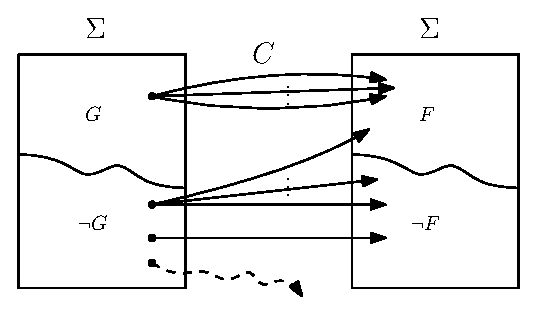
\includegraphics[width=0.7\textwidth]{image/wp-nondet.eps}
% \caption{Weakest Precondition (Angelic Non-determinism)}
% \label{fig:wp-nondet}
% \end{figure}

\begin{figure}[ht!]\centering
  \subfloat[wp (angelic non-determinism) \label{subfig:wp-angelic}]{
    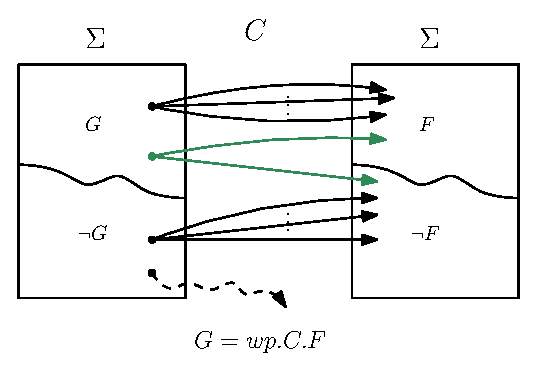
\includegraphics[width=0.45\textwidth]{image/wp-angelic.eps}
  }
  \hfill
  \subfloat[wlp (demonic non-determinism) \label{subfig:wlp-demonic}]{
    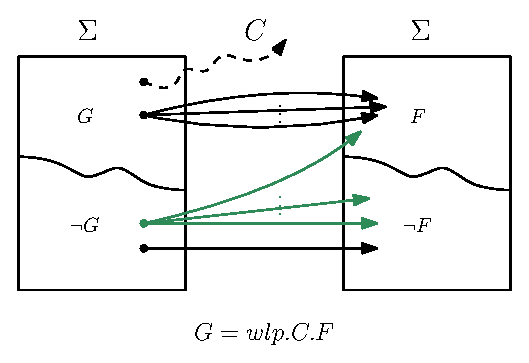
\includegraphics[width=0.45\textwidth]{image/wlp-demonic.eps}
  }
\caption{Weakest Precondition (Angelic Non-determinism) and Weakest Liberal Precondition (Demonic Non-determinism)}
\label{fig:wp-wlp-together}
\end{figure}



% To justify this definition for the non-deterministic choice, we must first clarify the intended semantics of the wp-transformer. 

% Let \mathl{\exec C} denote the \define{execution} of program $C$ and \mathl{\exec C.\sigma} denote the set of final states that \imptt{can} occur after the execution of $C$. 
% A state is a function that maps a program variable to a value. The set of \define{states} is denoted by \mathl{\Sigma=\{\sigma \mid \sigma: Vars\to Vals\}}. 

% If $C$ is deterministic, then $\exec C.\sigma$ is a set of a single state, either a final state $\sigma'$ or $\bot$, if the execution does not terminate. 
% If $C$ is non-deterministic, $\exec C.\sigma$ can be a set with multiple elements, since multiple final states can be possible. 

% The weakest precondition $wp.C.F$ is then 











\section{Weakest Liberal Preconditions}\label{sec:wlp}
While the wp-transformer excludes non-termination, the wlp-transformer takes a more liberal approach. 
The weakest precondition delivers a precondition so that the program terminates and a state satisfying the postcondition is \imptt{reachable}. 
The weakest liberal precondition, however, delivers a precondition so that the program either terminates satisfying the postcondition, or diverges. 
The postcondition in the wlp setting is \imptt{guaranteed} upon termination, because we regard the non-deterministic choice as demonic, again favoring to establish a Galois connection~\cite{zhang22}. 

We define the weakest liberal precondition transformer in \autoref{tab:wp-wlp}. 
A graphical representation can be found on \autoref{subfig:wlp-demonic}. 

As preluded earlier, greatest fixed points are used to define wlp for while-loops. 
It is an easy choice, since wlp is semantically the \imptt{weakest} liberal precondition, and $wlp.WHILE.F$ should be a fixed point of its characteristic function, similar to \autoref{sec:define loops}. 


%done{Explain the use of gfp. Possibly relate to page 185 of Dijkstra and Scholten 1990 book. }

% \begin{figure}[ht!]\centering
% 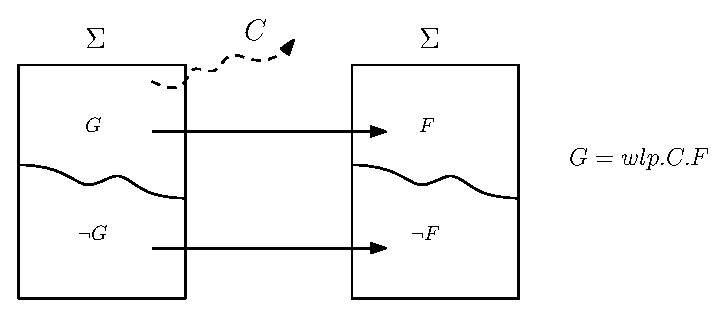
\includegraphics[width=0.7\textwidth]{image/wlp-det.eps}
% \caption{Weakest Liberal Precondition (Deterministic)}
% \label{fig:wlp-det}
% \end{figure}



\section{Strongest Postconditions}\label{sec:sp}
Following the style to define wp and wlp, Zhang and Kaminski~\cite{zhang22} (re-)defined \define{strongest postconditions} that capture the characteristics of all reachable states after the execution. 
In essence, $sp.C.G$ is a postcondition that is satisfied by \imptt{all} states that is \imptt{reachable} from $G$. 
The definition of the predicate transformer sp is shown in \autoref{tab:sp}. 

\begin{table}[ht!]\centering
    \begin{tabular}{l;{1pt/1pt}l}
    \hline\hline
      \textbf{C}&\textbf{sp.C.G}    \\ \hline
      $skip$&   $G$   \\ \hdashline[1pt/1pt]
      $diverge$&  $false$\\ \hdashline[1pt/1pt]
      $x:= e $&  $\exists a. x=e[x/a] \wedge G[x/a]$\\ \hdashline[1pt/1pt]
      $C_1;C_2$&  $sp.C_2.(sp.C_1.G)$\\ \hdashline[1pt/1pt]
      $\{C_1\}\square \{C_2\}$ & $sp.C_1.G\vee sp.C_2.G$ \\ \hdashline[1pt/1pt]
      $if\ (\varphi)\ \{C_1\}\ else\ \{C_2\} $&  $sp.C_1.(\varphi\wedge G)\vee sp.C_2.(\neg\varphi\wedge G)$\\ \hdashline[1pt/1pt]
      $while\ (\varphi)\ \{C'\}$&  $\neg\varphi \wedge lfp\ X. G\vee sp.C.(\varphi\wedge X)$\\
    \hline\hline
    \end{tabular}
    \caption{The Strongest Postcondition Transformer~\cite{zhang22}}
    \label{tab:sp}
\end{table}

We can also illustrate the behavior of a program controlled by sp in \autoref{fig:sp-angelic}. 
Instead of discussing termination starting from a precondition, sp focuses on reachability of states satisfying postconditions. 
The dotted arrow points to postconditions describing unreachable final states after the execution of $C$. 
For example, no state would satisfy $x=2$ after the execution of $x:=1$. 

\begin{figure}[ht!]\centering
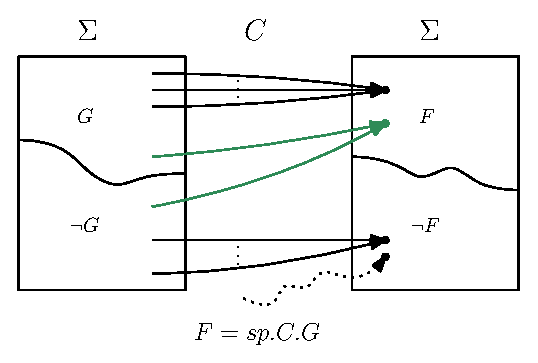
\includegraphics[width=0.45\textwidth]{image/sp-angelic.eps}
\caption{Strongest Postcondition (Angelic Non-determinism)}
\label{fig:sp-angelic}
\end{figure}




\section{Soundness}
\begin{theorem}{wp-sound}[Soundness of wp]~{\normalfont\cite{zhang22}} 
\ \vspace{-1.5mm}
\[
wp.C.F = \{\sigma\in\S \mid \neg(\sigma\goto{C}\bot)\ \wedge\  \exists \tau\in\S.\, \sigma\goto{C}\tau: \  \tau\vDash F\}
\]
\end{theorem}

\todo{make sure the theorem and its content is on the same page}
\begin{theorem}{wlp-sound}[Soundness of wlp]~{\normalfont\cite{dijkstra90}}
\ \vspace{-1.5mm}
\[
wlp.C.F = \{ \sigma\in\S \mid
\sigma\goto{C}\bot \ \vee\ 
\forall \tau\in\S.\, \sigma\goto{C}\tau:\  \tau\vDash F
 \}
\]
% \label{thm:wlp}
\end{theorem}

\begin{theorem}{sp-sound}[Soundness of sp]~{\normalfont\cite{vries11,zhang22}}
\ \vspace{-1.5mm}
\[
sp.C.G = \{ \tau\in\S \mid \exists \sigma\in\S.\, \sigma\goto{C}\tau: \  \sigma\vDash G\}
\]
\label{thm:sp}
\end{theorem}


\section{Properties of wp and wlp}
wp and wlp are each other's conjugate: 
\[wp.C.F = \neg wlp.C.\neg F\]

% \[wp.C.false = false\]
% \[wlp.C.true = true\]
% \[wp.C.true = preconditions that lead to termination\]
% \[wlp.C.false = preconditions that lead to non-termination\]


\textbf{[TO BE CONTINUED]}


%*****************************************
%*****************************************
%*****************************************
%*****************************************
%*****************************************
